\newcommand{\TimingRows}{%
Emma & 4,096 & 0.314 & 0.16 & 1.327 & 1.12 & 2.44 \\
Moby-Dick & 4,096 & 0.246 & 0.16 & 0.460 & 1.05 & 1.50 \\
Emma & 32,768 & 2.084 & 0.69 & 4.657 & 2.89 & 7.54 \\
Moby-Dick & 32,768 & 2.077 & 0.69 & 3.783 & 2.88 & 6.66 \\
Emma & 131,072 & 9.184 & 2.45 & 15.937 & 10.00 & 25.93 \\
Moby-Dick & 131,072 & 9.203 & 2.46 & 14.931 & 10.01 & 24.94 \\
}


\section{GPU protocol and measured timings}
\label{app:record}
\paragraph{Runtime.}
The trace records PyTorch 2.14.1+cu130, CUDA 13.0, Triton 3.8.0, FlashInfer 0.7.5.post1 and Transformers 5.5.0. The model revision is \texttt{2fc06364715b967f1860aea9cf38778875588b17}. Full-attention layer indices are 3, 7, 11, 15, 19 and 23 (zero-based). For the recurrent layers the reported decode function is \texttt{torch\_recurrent\_gated\_delta\_rule}. The reader uses four warps, one pipeline stage, and a split attention calculation followed by a reduction. The two backends share a fused gate/output projection. Weights, recurrent state, workspaces, status flags and allocator overhead are outside the reported KV capacity. In particular the compact partial-output and softmax-statistic buffers consume additional device memory.

\paragraph{Timing and aggregation.}
Disclosure of the timing boundary matters for a sub-percent effect. The clock starts after cloning recurrent state and synchronizing the GPU. Each call to \texttt{item()} makes the selected ID available on the host. A final synchronization precedes the end timestamp. Each backend reuses its built decoder across runs; suffix slots are overwritten and only the valid prefix plus current suffix is visible. The alternating order starts with a different backend on the two books at each context length. A pair's plotted change is $100(t_{\rm dense}/t_{\rm compact}-1)$ because token counts match. Pooled rates weight elapsed time by summing tokens and seconds before taking their ratio. Error ranges in the paired plot show all four observed ratios; they are not confidence intervals. The 48 timed runs total 38.52 seconds of generation. This excludes data loading, build, prefill, warm-up, probes and compilation outside the timers. The complete project-wide GPU-hour total was not logged.

\begin{table}[ht]
\centering
\caption{Measured prefill and build times, with reconstructed single-request totals. Dense build is reported in milliseconds; all other time columns use seconds. Totals add common prefill, method-specific build and the mean of four warm runs of 64 tokens. They exclude unrelated setup and compilation outside these stages.}
\label{tab:stage}
\begin{tabular}{lrrrrrr}\toprule
Book & Prefix & Prefill & Dense build & Compact build & Dense total & Compact total\\
 & (tokens) & (s) & (ms) & (s) & (s) & (s)\\\midrule
\TimingRows
\bottomrule\end{tabular}
\end{table}

\begin{figure}[ht]\centering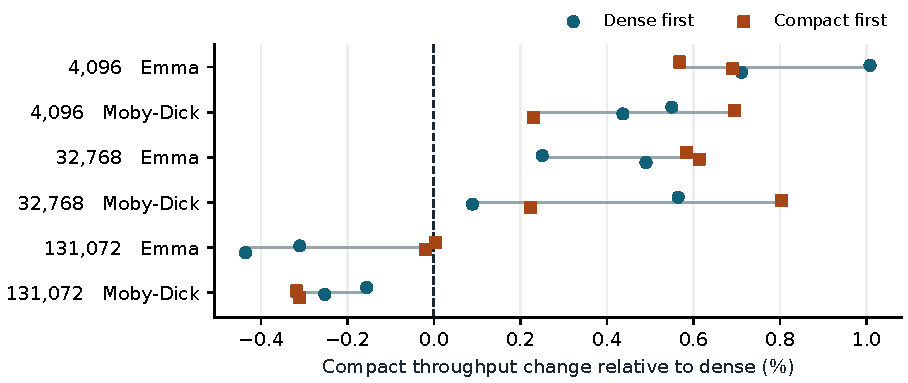
\includegraphics[width=.93\linewidth]{figures/paired.pdf}
\caption{The 24 within-condition timing pairs. The line spans the observed range, and the symbols give the order of the dense and compact runs. Positive change favors compact storage.}\label{fig:pairs}
\end{figure}
\paragraph{Where fallback occurs.}
Figure~\ref{fig:fallback} counts 768 appended rows per tensor and layer: two groups, 64 new positions and six conditions. Each condition contributes once. The value fallback changes from $0/768$ at layer 7 to $764/768$ at layer 23. These counts explain variation in logical suffix size. Reserved suffix capacity is independent of the fallback count. For the six layers in order, the recorded maximum absolute row sums of $W$ are 61.05, 36.40, 40.34, 38.46, 49.36 and 40.61 (rounded). In particular the final layer does not have the strictest nominal coordinate tolerance. These records alone cannot distinguish the effects of the realized exponent ranges and rounding residuals on each row.

\begin{figure}[ht]
\centering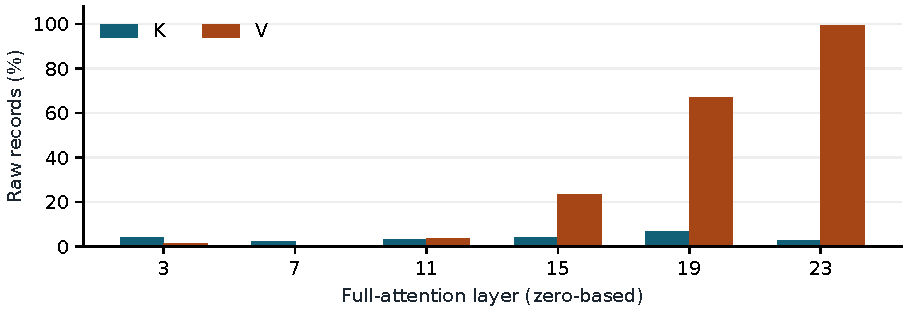
\includegraphics[width=.90\linewidth]{figures/fallback.pdf}
\caption{Fraction of appended records that use the full BF16 payload. Counts pool the six distinct prompt-length conditions, without counting timing repetitions. K and V use different fallback criteria.}
\label{fig:fallback}
\end{figure}

\paragraph{Independent arithmetic and integration checks.}
On a short prefix of 255 tokens, a separate probe compares each custom decode path with the original Hugging Face text decoder over four common-history steps, crossing the 256-position boundary. All eight backend--reference top choices agree. This checks integration at four positions only; the long-context dense baseline is the FlashInfer path described in the main text. The supplied CPU reference additionally exercises exact key round trips and four value budgets on 244 synthetic BF16 rows, including signed zeros, subnormals and wide exponent spreads. The corresponding script records the seed and tests raw as well as packed values. The long-context logits and continuations reported above come solely from the archived GPU trace.

\paragraph{Reproducing the paper.}
The artifact contains the measured JSON, model revision, corpus and token hashes, per-token times, generated IDs, verification scripts and GPU kernels. The CPU replay re-derives the tables, the three vector figures and the allocation identities. The optional fresh run uses a compatible NVIDIA stack, fetches the two source books and verifies their hashes. A new run writes to a separate location so the published measurements retain their identity. One source archive compiles with pdfLaTeX and includes the figures as PDFs. The notebook embeds the experiment scripts, CPU replay inputs and plotting code.

\paragraph{Scope, assets and disclosure.}
Qwen supplies the checkpoint under Apache-2.0. NLTK lists its Project Gutenberg selections as public domain; the companion retrieves upstream texts by hash and distributes neither books nor model weights. The benchmark concerns infrastructure for inference. Reducing cache storage could lower the cost of some deployments; increased capacity can also increase total use. The measurements contain no energy or emissions data. No human participants or personal evaluation records are involved. Generative AI assisted in drafting the analysis, deriving the mathematical presentation, writing verification and packaging code, and preparing the manuscript. The measurement claims are tied to the supplied run record.
